\documentclass[preprintnumbers,amsmath,amssymb,superscriptaddress,twocolumn,showpacs]{revtex4-1}
%\documentclass[preprintnumbers,amsmath,amssymb]{revtex4}
\usepackage{graphicx}% Include figure files
\usepackage{dcolumn}% Align table columns on decimal point
\usepackage{bm}% bold math
\usepackage{natbib}
\usepackage{physics}
\usepackage[caption=false]{subfig}

%\newcommand{|}{Y$_2$SiO$_5$}
\def\sgn{\mathop{\rm sgn}}
\newcommand{\be}{\begin{equation}}
\newcommand{\ee}{\end{equation}}
\newcommand{\bea}{\begin{eqnarray}}
\newcommand{\eea}{\end{eqnarray}}

\begin{document}

\title{Mechanical Detection of Dipole-Dipole Interactions \\between Electronic Spins in a Solid}

\author{C. Pellet-Mary, P. Huillery, M. Perdriat, G. H\'etet} 

\affiliation{$^1$Laboratoire Pierre Aigrain, Ecole normale sup\'erieure, PSL Research University, CNRS, Universit\'e Pierre et Marie Curie, Sorbonne Universit\'es, Universit\'e Paris Diderot, Sorbonne Paris-Cit\'e, 24 rue Lhomond, 75231 Paris Cedex 05, France.}

\begin{abstract}
Magnetic-dipole interactions between the spins of defects in crystals play a key role in a vast range of applications. In typical experiments on nuclear or electronic spin resonance, the interactions are identified in the electromagnetic emission or absorption spectrum of the spins.
Here, we demonstrate mechanical detection of dipolar interactions. 
Using a levitating diamond containing nitrogen-vacancy (NV) centers, we employ cross-relaxation to alter 
the spin-torque when pairs of NV centers' orientations become resonant.
Our approach opens a path towards the use of mechanical oscillators to detect paramagnetic defects that lack optical transitions. 
\end{abstract}

\maketitle

Defects in solid state materials with long-lived electronic or nuclear spins play a key role in the fields of quantum computing, communication and sensing. 
Such defects can be hosted by various materials, the most studied examples being nuclear impurities in quantum dots \cite{Qdots}, dopants in silicon \cite{Zwanenburg}, or negatively charged nitrogen vacancy (NV$^-$) centers in diamond \cite{Doherty}.
The detection of their spins is generically performed {\it via} emission or absorption of electromagnetic radiation, both in the radio/micro-wave or optical domain, or purely electrically \cite{Zwanenburg, Hopper}.
Electron-Paramagnetic Resonance (EPR) and Optically Detected Magnetic Resonance (ODMR) are two such detection methods, both routinely operating under ambient conditions and with large signal to noise ratios.
EPR can detect most paramagnetic species with great accuracy, while the latter reaches single spin resolution \cite{Wrachtrup1}, albeit only with optically active defects.
Notably, both techniques can also efficiently detect spins through magnetic dipolar interactions. 
Dedicated Pulsed-EPR \cite{Mims} and ODMR protocols such as the Double-Electron-Electron-Resonance (DEER), Electron-Nuclear-Double-Resonance (ENDOR) or Cross-Relaxation (CR) at the Hartmann Hahn resonance have all indeed been proven essential for characterizing dipolar interactions, offering ways to detect distant spins \cite{Mamin}.

Another more recent route for detecting spins is to couple them to mechanical oscillators.
Electronic spins have first been detected this way in \cite{Alzetta} and nuclear spins can be sensed using state of the art magnetic resonance force microscope (MRFM) \cite{rugar, MaminH}. MRFM is a very efficient probe for paramagnetic impurities with nanometer resolution.
Conversely, torque sensors lends themselves naturally to the detection of solid state defects, which thanks to anisotropic terms in the spin hamiltonian can exert torques in a homogeneous magnetic field. 
Torque sensing was employed recently to detect the long-lived spins of NV centers in diamonds and to demonstrate spin-cooling of a mechanical oscillator \cite{DelordNat}.
In general, spin-mechanical experiments with long-lived spins also offer prospects for performing quantum mechanical experiments with large objects \cite{yin, Wan, Scala, Lee_2017}. However, while dipolar interactions can be detected using EPR or ODMR, mechanical detection of dipolar interactions between long-lived spins has not been observed. Compared to these two established techniques, it could offer the advantage of sensing angular momentum conservation during dipolar relaxation \cite{Zangara} as well as providing an alternative path for controlling the quantum motion of mechanical oscillators.

Here, we report on the detection of spin-interactions using a mechanical torque sensor.
Specifically, we employ a levitating diamond in a Paul trap with embedded NV centers and use the diamond orientation as a probe of the NV spin interactions.
%We use closely packed nitrogen-vacancy centers to ensure both large spin-torques on the mechanical oscillator together with large dipolar-interactions amongst the spins.

%When this occurs, the spin-torque is modified so that subsequently, the diamond rotates.

\begin{figure}[!ht]
  \centering \scalebox{0.45}{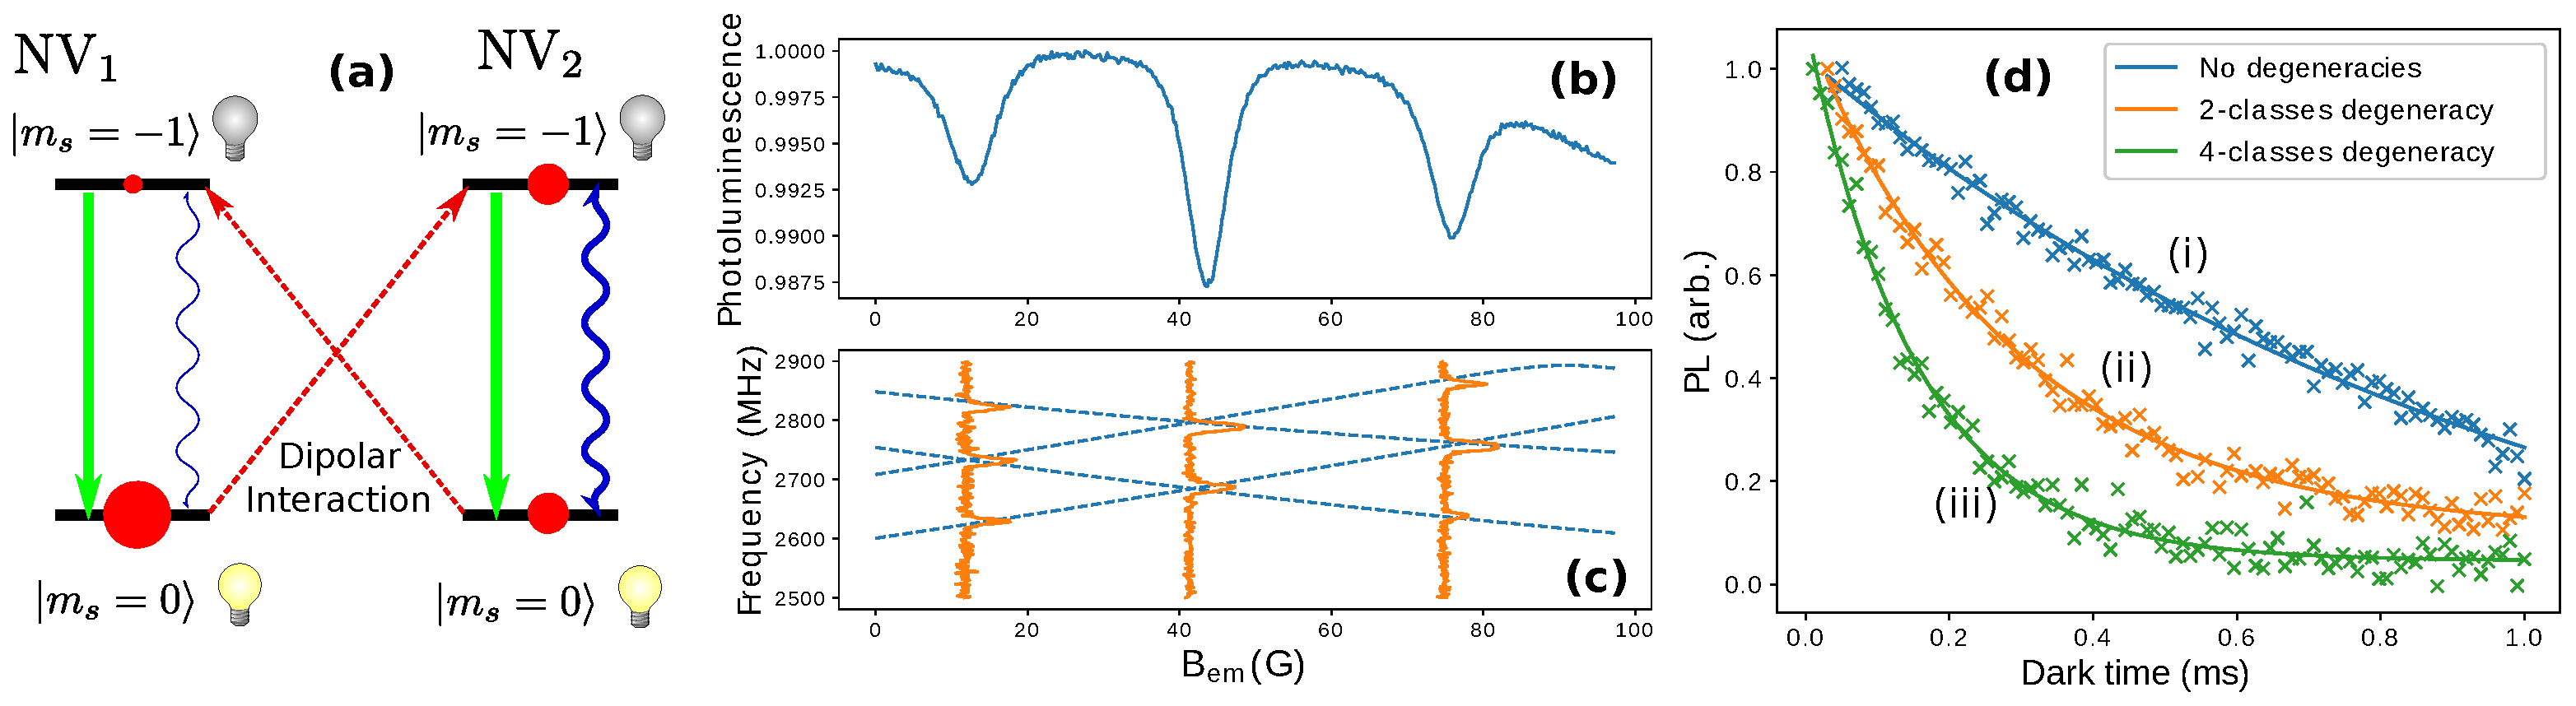
\includegraphics{Adamas_fixe.eps}}
  \caption{a) Photoluminescence signal in function of the scanning magnetic field. b) Predicted transition frequencies for the four classes of NV centers (dashed). ESR spectra for particular value of the magnetic field (plain, vertical)}
  \label{CR_deposited}
\end{figure}


\begin{figure}[!ht]
  \centering \scalebox{0.5}{\includegraphics{T1.eps}}
  \caption{Longitudinal relaxation from a single class of NV centers with exponential fit. i) The class is not at resonance with any other classes : T$_1$=1.02 ms. ii) The class is at resonance with another class : T$_1$=0.28 ms. iii) The class is at resonance with the three other classes : T$_1$=0.15 ms.
  }\label{T_1}
\end{figure}

%We first present the results and conclude by discussing the potential applications behind our observations.
The key idea of our mechanical detection of dipolar interactions lies in the cross-relaxation (CR) that takes place when two spins with different orientations and polarization become resonant. This can be achieved by tuning a magnetic field when using spin-1 defects such as the NV center.
The NV center has two electrons in the ground state, and a zero-field splitting $D=2.87$ GHz.
The ground states are labelled $| m_s={0}, {\pm 1}\rangle$.
Due to an intersystem crossing in the excited state of the NV centers \cite{Doherty}, the state $m_s=\ket{0}$ is brighter than the state $m_s=\ket{\pm 1}$ upon green laser optical illumination \cite{Hopper}. This provides a means to read out the Zeeman splitting by scanning a microwave tone around the resonance, carrying out ODMR.

The diamonds that we use are in the form of a powder of particles that have a diameter of 15 $\mu$m. They are supplied by the company Adamas, which produces diamonds with a concentration of NV centers in the 3-4 ppm range. 
We operate with a Paul trap that is similar to the one used in \cite{delordPRL} with particles are stably trapped at the bottleneck region, where both the electric field gradient and anisotropy are stronger.
The microwave is applied directly on the trapping electrode, which provides an efficient means to excite the spins.
The photoluminescence is detected using standard confocal microscopy. We use about 100 $\mu$W of laser light at 532nm to polarise the NV centers. The laser is focused via a lens inside the vacuum chamber which has a numerical aperture of 0.5 and a working distance of 8mm. The focal point of the laser is kept few tens of micrometer away from the micro-diamond to mitigate the effect of radiation pressure and to enable laser excitation of the whole diamond \cite{delordPRL,delord2016}. 

Let us first show that dipolar interaction in our diamonds is effective by studying cross-relaxation with diamonds that are simply attached to the trap.
In diamonds that contain more than 1 ppm of nitrogen-vacancy centers cross relaxation effects have been observed by many groups \cite{van_oort_cross-relaxation_1989, armstrong_nvnv_2010, jarmola_longitudinal_2015, akhmedzhanov_microwave-free_2017, akhmedzhanov_magnetometry_2019, holliday_optical_1989, mrozek_longitudinal_2015, jarmola_temperature-_2012, choi_depolarization_2017}.
It manifests itself as a change in the longitudinal relaxation rate of NV centers, which can then translate as a reduction of the overall photo-luminescence. 

This effect has been routinely observed in bulk materials, the origin of which was attributed to the presence of charge tunneling amongst closely packed NV centers \cite{choi_depolarization_2017}. The NV centers that undergo tunneling with other impurities (possibly the substitutional nitrogen defect \cite{Manson}) have a reduced longitudinal spin lifetime $T_1$. When their energy matches the energy of NV centers that have phonon-limited lifetimes ($T_1\approx 5 ms$), the latter can drop 
to a few hundreds of micro-seconds \cite{Jarmola} when the NV concentration is large enough (typically in the ppm range)
This process has recently revived interest recently because the sensitivity of magnetometers is ultimately limited by these interactions \cite{Zhou}. 
%In our spin-mechanics experiment, we use micro-diamond particules subjected to a green laser field and a magnetic field.
%To observe the dipolar effects in a levitating platform, we employ heavily doped micro-diamonds.
In our experiment, we first probe CR by using a fixed bias magnetic field $\bf B_{\rm bias} \approx$ 100 G and scan another magnetic field $\bf B_{\rm em}$ at some angle with $B$ using an electromagnet. 
Figure \ref{CR_deposited}-a) shows the photoluminescence from the NV centers as a function of $\bf B_{\rm em}$. 
For these measurement we use a 1 mW green laser excitation which yields a repolarisation rate of about 100 $\mu$s. 
Three dips in the fluorescence can be observed. 
We attribute these to cross-relaxation that takes place when two orientation meet. To be sure, we recorded Electronic spin resonance spectra for different values which allows us to measure the total magnetic field felt by the spins, and therefore to extrapolate the transition frequencies of the four classes of NV for any applied $\bf B_{\rm em}$.
There is indeed a strong correspondence between the PL dips and the degeneracy conditions. 
(See SI for details on planes that cross etc.). 
We tentatively attribute those to CR. 
%It is important to characterize this effect further when using smaller particles such micro-diamonds where surface effects can play a role. 
%where, to our knowledge, such cross-relaxations have not been observed. 
%Indeed, surface effects may start to play a role and change quantitatively. 
To confirm our interpretation, and to extract the spin-torque dynamics in the mechanical experiment, we measure the longitudinal relaxation time ($T_1$ time) of the NV spins under different degeneracy conditions.

The measurement consists in applying a green laser to polarize the NV centers and to measure the photoluminescence at a later time. 
Such a measurement turns out to be hidden by recharging of NV centers in the dark, as has been observed and analyzed by several groups \cite{choi_depolarization_2017, mrozek_longitudinal_2015, giri_selective_2019, giri_coupled_2018}.
In order to accurately measure the $T_1$ and remove the changing PL due to the recharging effects, we use a sequence presented in the SI, where a microwave pulse is applied or not prior to relaxation. Subtracting the two resulting signals eliminates charge dynamics from the spin decay.
The results of the measurements are shown in Fig. \ref{T_1} for different degeneracies. 
It can be seen that $T_1$ is greatly shortened, from X to Y when approaching degeneracy, confirming this interpretation.

\begin{figure}[!ht]
  \centering \scalebox{0.13}{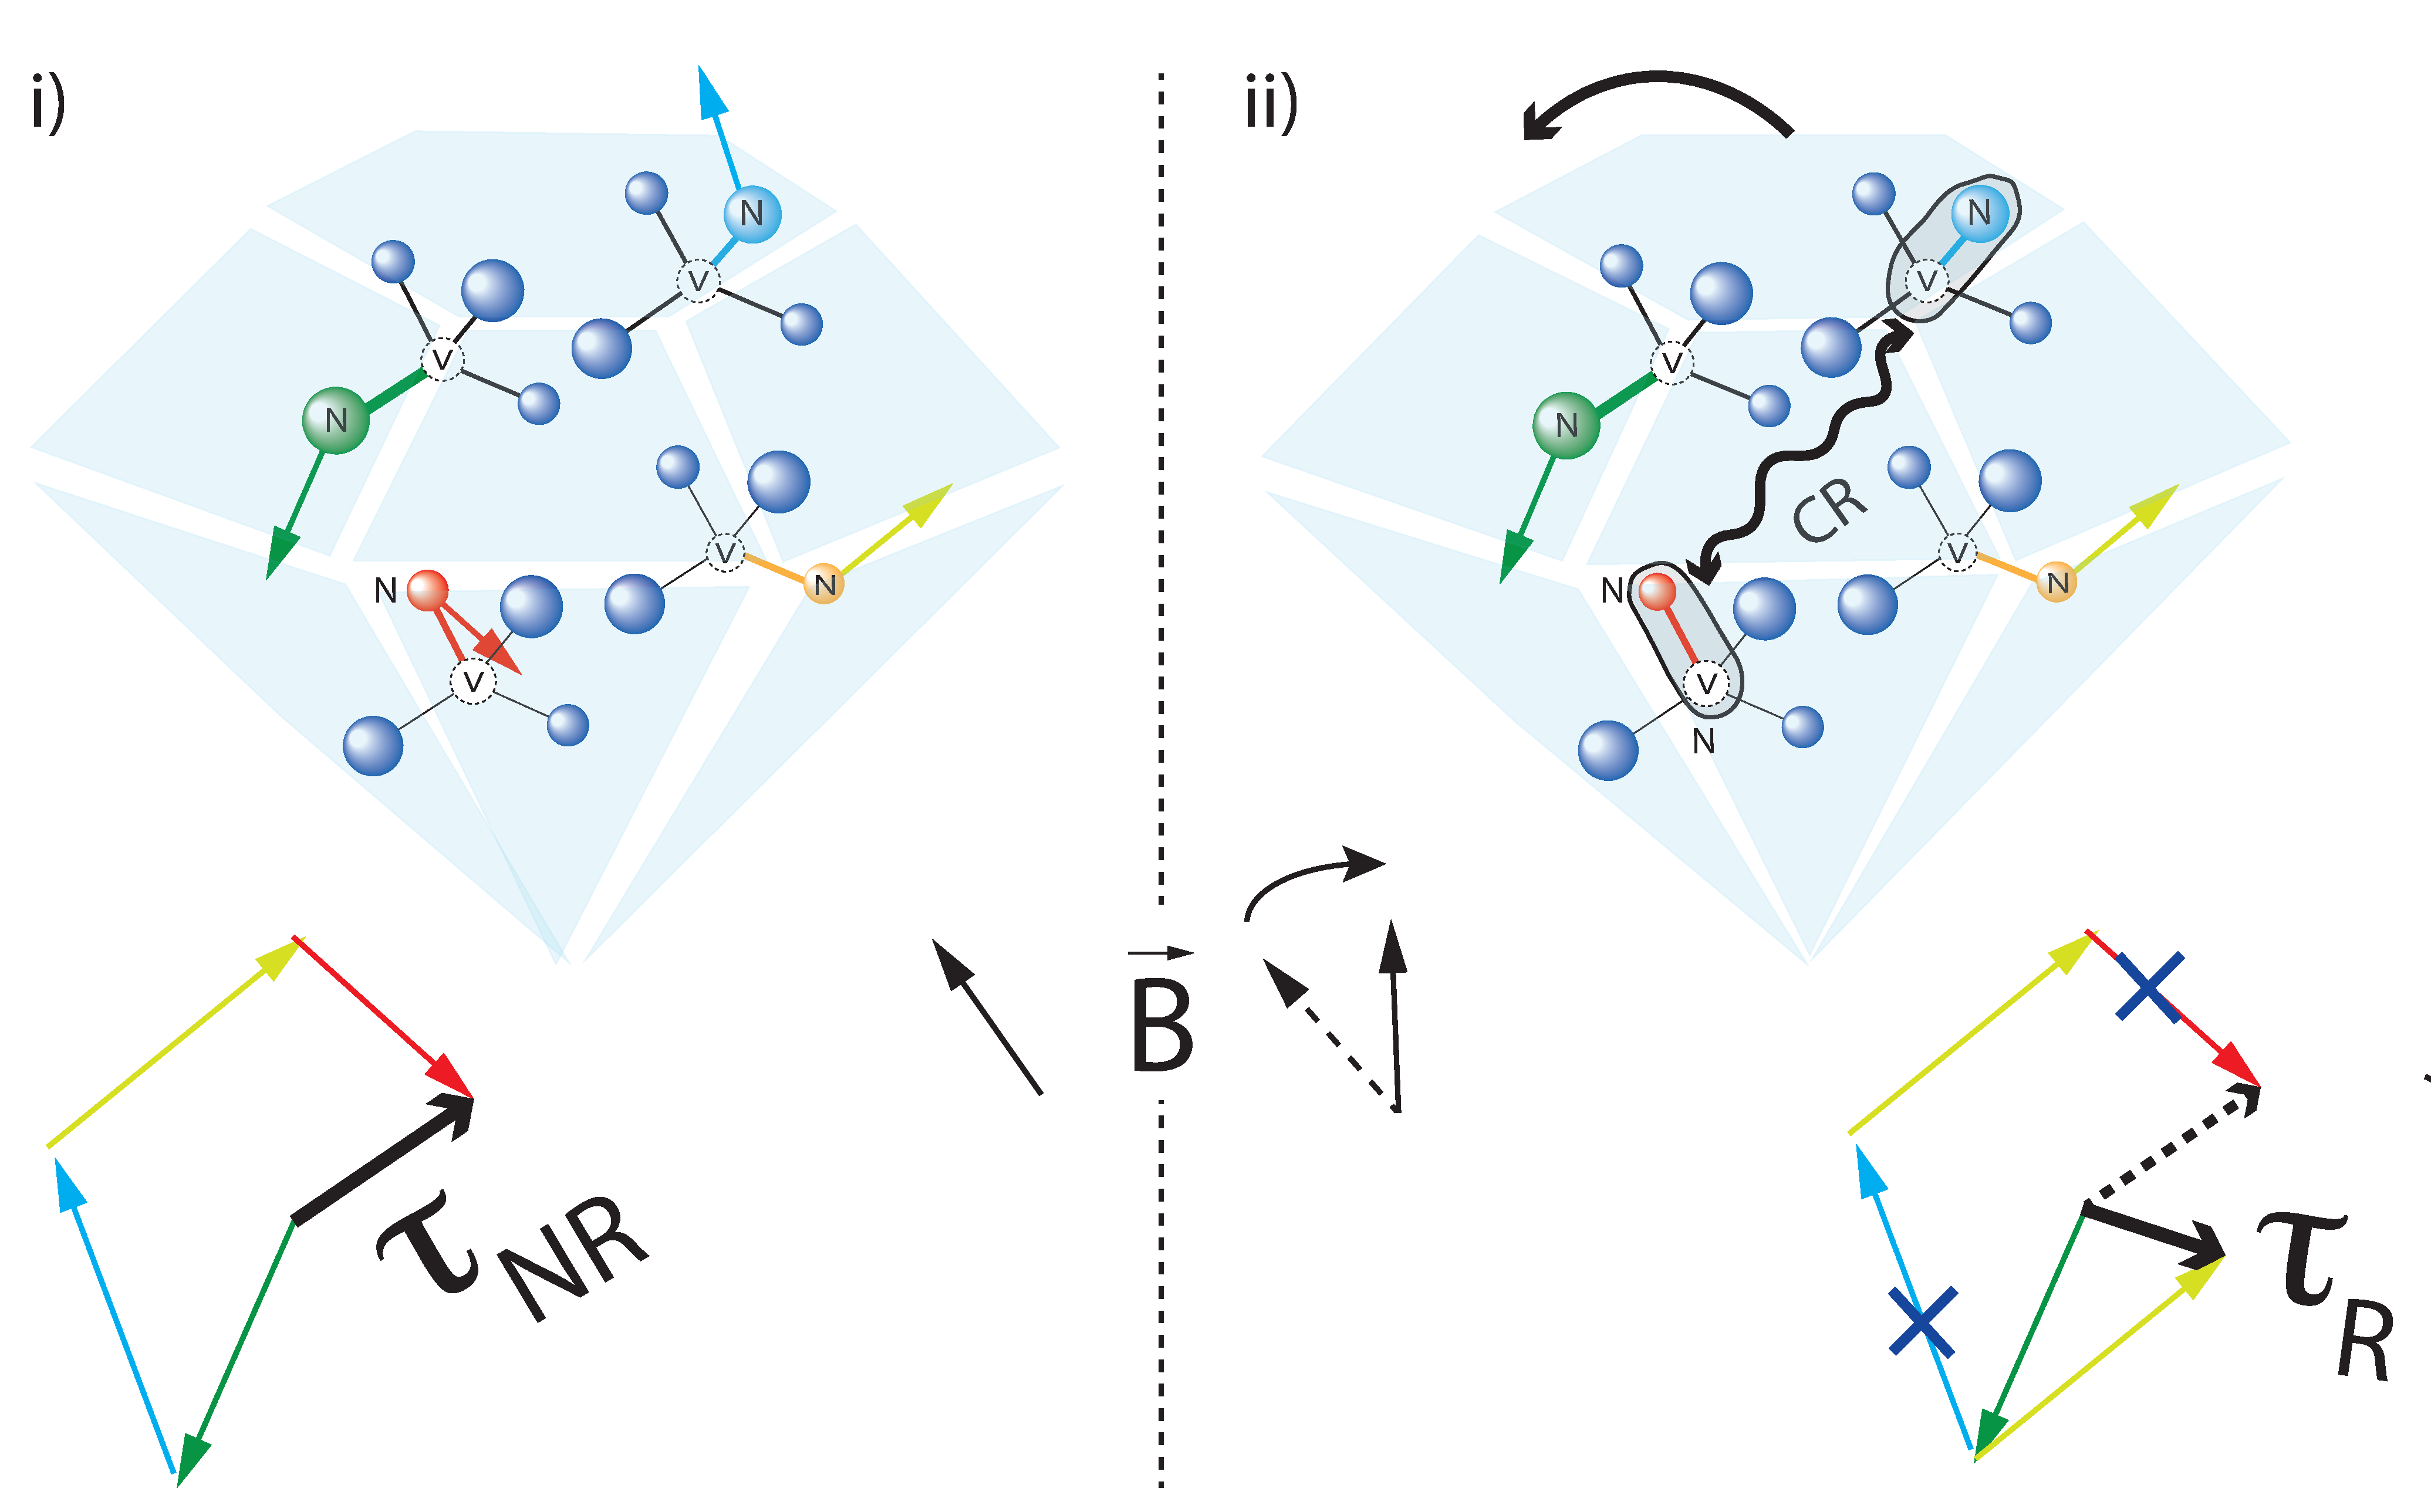
\includegraphics{dilutednv.pdf}}
  \caption{Sketch showing the principle of the mechanical detection of the dipolar-interaction i): Depiction of the four possible $<111>$ directions of Nitrogen (blue, green yellow and red balls) vacancy (white) centers in the diamond crystalline structure. Here, the magnetic field is tuned so that no cross-relaxation can occur.
The resulting non-resonant spin-torque $\tau_{NR}$ applied to the levitating diamond is sketched below. 
ii) Here, the magnetic field is tuned so that cross-relaxation can occur between two classes of NVs.
The resulting resonant spin-torque $\tau_{R}$ applied to the levitating diamond (below) is thus modified. 
  }\label{principle}
\end{figure}

%
%\begin{figure}[!ht]
%  \centering \scalebox{0.6}{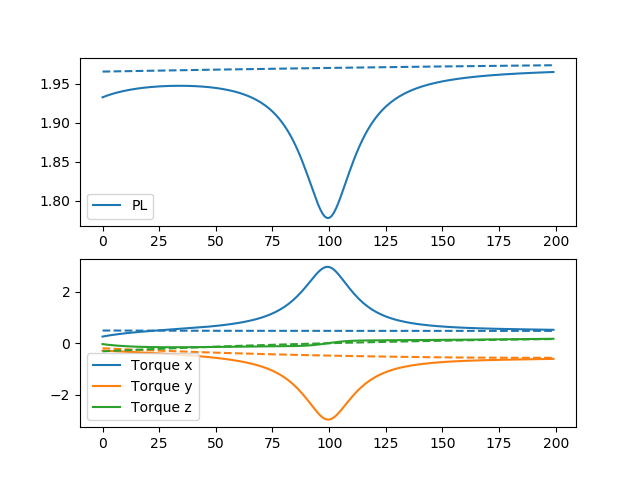
\includegraphics{cross_121_200G.png}}
%  \caption{Numerics : PL change in the presence of cross-relaxation (top) and spin-mechanical detection (below). 
%  }\label{CR_deposited}
%\end{figure}

Let us now study these heavily doped diamonds in the trap, with the goal to mechanically detect the dipolar interactions.
Specifically, we will detect the diamond angle and seek for changes in the diamond orientation at CR conditions. The detection is optimized by collecting the back reflected green light from the diamond interface, separated from the excitation light using a polarizing beam splitter. The best sensitivity is achieved by using a speckle pattern produced by the rough surface of the micro-diamond under coherent illumination. When the particle is stably levitating, at the particle image plane, a speckle feature is formed. To detect the diamond motion, we then focus a small area of this image onto an optical fibre and detect the photons transmitted through the fibre with a single-photon avalanche photodiode. The detected signal is then highly sensitive to the particle position and orientation.

%For a given levitating particle, we can optimize, in real time, the signal coming from the angular displacement of the particle by selecting the most favorable region of the particle image. To do this, we monitor our optical signal while switching a microwave field tuned to one of the ESR transitions, at a frequency of 1 Hz.  Alignment is realized by maximizing the variation of the coupled light as the diamond rotates between two angular positions. 

One major ingredient of the present study compared to \cite{DelordNat} is the spin-torque coming from the NV centers in the absence of the microwave tone.
For this, let us consider first the torque coming from a single spin due to the transverse component of the magnetic field when the NV is in the ground state.
The hamiltonian for one NV orientation with quantization axis $z$ reads 
\begin{equation}\hat{H}_{\rm NV}=\hbar D \hat{S}_z^2+ \hbar \gamma_e \bf B  \cdot \bf\hat S.
\end{equation}
Under the condition $\gamma B \ll D$, $H_{B}= \gamma_e B  ( S_x \cos\theta + S_z \sin\theta)$ can be treated as a perturbation to the anisotropic part of the hamiltonian. 
The perturbed energy $\epsilon_g$ of $\ket{0}$ due to the transverse B field is then
\begin{equation} \epsilon_g=\sum_{m_s=\pm 1}\frac{ |\bra{0} H_B \ket{\pm 1}|^2}{-\epsilon^0_{\pm 1}}=-\hbar\frac{(\gamma_e B)^2 }{D} \cos^2\theta.
\end{equation}
One can deduce the total torque when N spins of a given orientation are polarised in the ground state to be 
\begin{equation}\tau_g=-N \frac{\partial \epsilon_0}{\partial \theta}=\hbar N  \frac{(\gamma_e B)^2}{D} \sin 2\theta.\end{equation}

At an angle $\theta=\pi/4$, where the torque is maximized, using $10^9$ spins polarized in the ground state and a B field of 100 G, the static torque is about $10^{-19}$ N.m.
We checked numerically that at these magnetic field values and angle, the NV are still polarized mostly in the ground state. 
Note that the torque is zero at $\theta=mod (\pi/2)$ where the eigenstates of $S_z$ are not mixed. The hamiltonian ground state is the eigenstate $| S=1,m_s=0\rangle$, which is is non magnetic. 
%Note also that the torque tends to zero if  tends to zero at any angle $\theta$. This is the case in the presence of strong spin-depolarisation, i.e. when $\hat\rho\rightarrow\frac{1}{3}\hat{I}$ (with $\hat{I}$ the identity operator).

Although the physics of the torque differs from the torque observed in \cite{DelordNat}, which came from the microwave excitation to magnetic states, this torque is comparable in magnitude. With our angular resolution of 100 $\mu$rad/$\sqrt{\rm Hz}$, it should thus enable a measurable shift in the angular position to be detected and possibly modified when cross-relaxation occurs. 
One major difference however, compared to \cite{DelordNat} is that the microwave selectively excited one class only. 
Here, we are interested in the modification of the total torque in the NV ground state, where all the NV orientation play a role. We thus also need to evaluate their contributions.
When estimating the total torque including the four classes, we found (see SI) that is is one order of magnitude weaker than for the above single class estimate.

\begin{figure*}[!ht]
  \centering \scalebox{0.45}{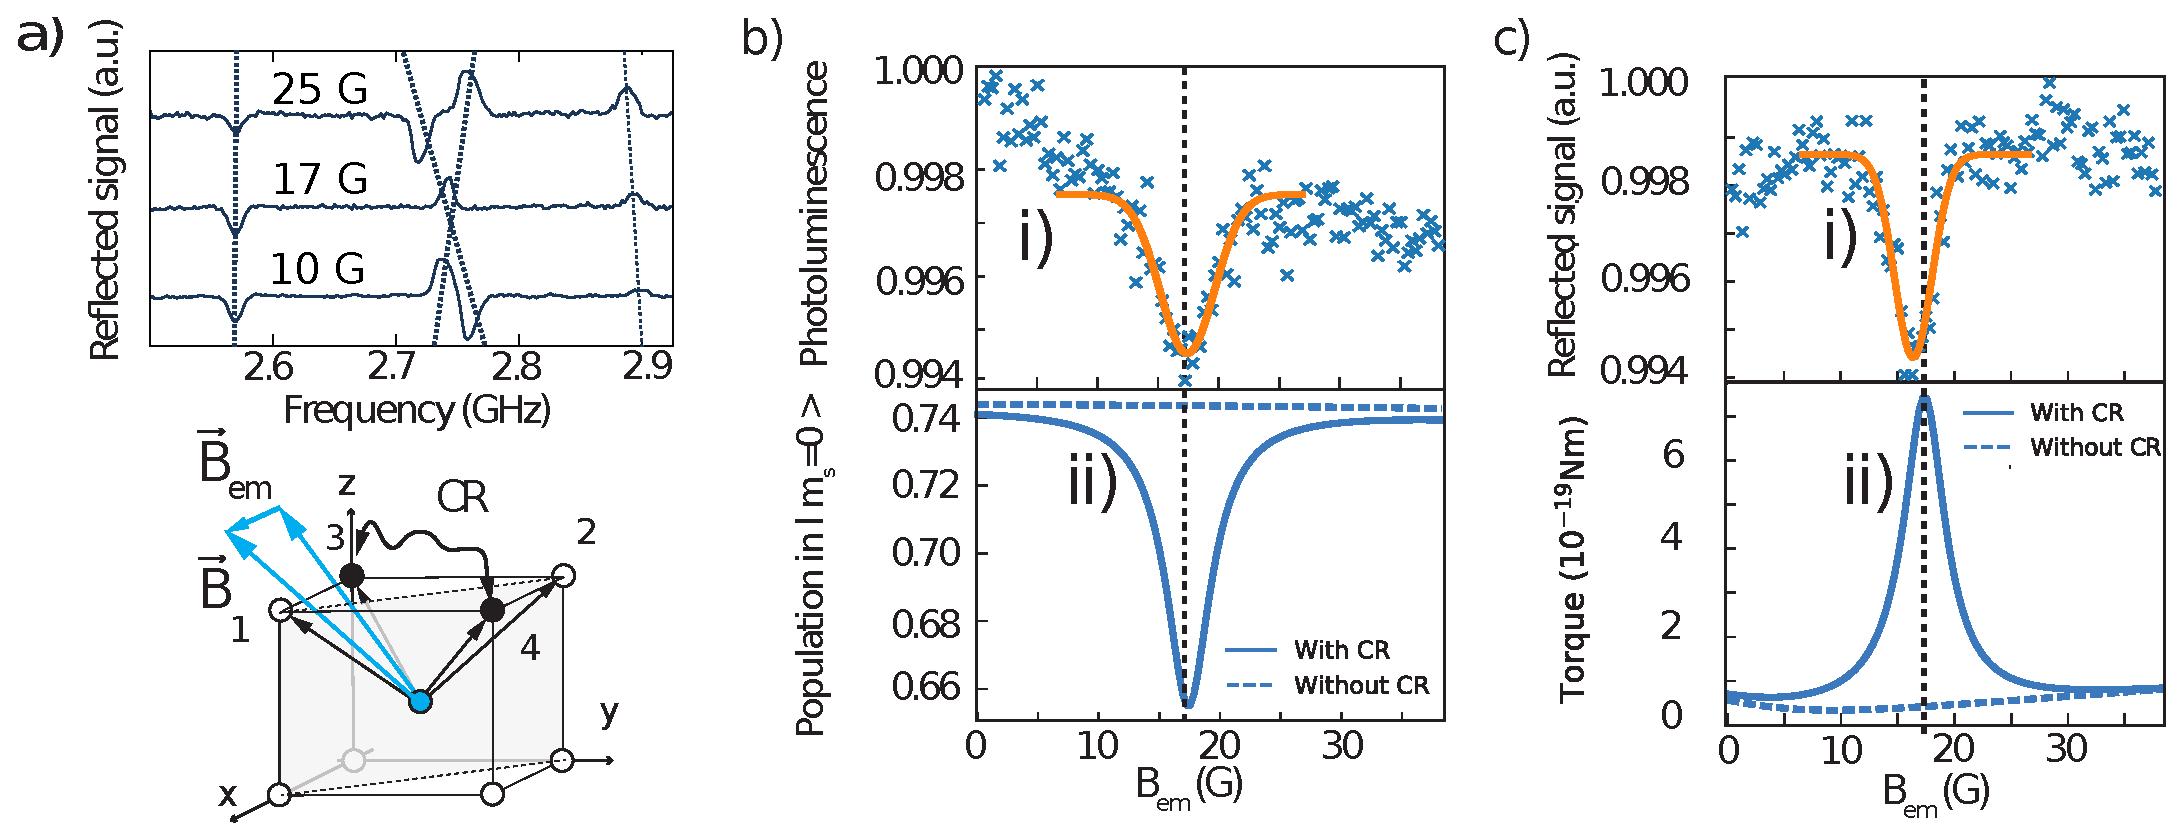
\includegraphics{CRmeca}}
  \caption{a) Angular detection of the diamond as a function of microwave frequency for three different magnetic field values. 
b) PL detection as a function of B$_{em}$ across a co-resonance. trace i) exp, trace ii) theory. 
c) Angular detection... 
  }
  \label{data}
\end{figure*}

Let us now explain why CR modifies the NV spin torque.
Fig. \ref{principle}-i) is a depiction of a levitating diamond containing NV centers that have four possible directions along the $<111>$ axes. 
In the presence of a magnetic field, each NV centers has a different magnetic field projection, which means a different torque. 
Below, we show the sum of the ground state spin-torques $\tau_{NR}$, resulting from the four classes. 
Fig. \ref{principle}-ii) shows the same situation, with a magnetic field that is tuned so that two NV classes are co-resonant. 
When the re-polarisation rate due to the green laser is smaller than the cross-relaxation rate, the magnetization coming from these two classes (indicated by a circle) tends to cancel. The population in the three NV eigenstates will indeed equilibrate, giving a smaller magnetization.
The resulting torque is thus changed to $\tau_{R}$ and the diamond then turns about another angle.
This is the essence of the proposed dipolar detection. 

%shows the total torque when 1-2-3-4 NV transitions are in the ground state. It is very small because the torque from 
%2-4 and 1-3 cancel each other. Looking at each pair 2-4 and 1-3 however, one can see that the torque is large (here 20 MHz for one spin).

To observe this effect we use similar parameters and magnetic field arrangement than when the diamonds where outside the trap.
Let us first monitor the spin-mechanical resonances. 
Fig. \ref{data}-a) shows the signal coming from the laser reflected off the diamond surface as a function of the microwave signal driving the NV centers' spins, with a zoom on the $m_s=-1$ states frequencies.
Three ESR have been taken for three different $\bf B_{\rm em}$ amplitudes. 
At 10 and 25 G, one can observe 4 pics in the spectrum, that are demonstrate spin induced torque on the diamond from the 4 classes of NVs.
At 17 G however, two classes merge at 2.75 GHz. This is where we expect CR.

Analysis (SI) suggest that we cross a single degeneracy that is the magnetic field crosses a $(110)_\perp$ plane.
 Fig. \ref{data}-b) shows the photoluminescence as a function of $\bf B_{\rm em}$ both experimentally (trace i) and numerically (trace ii)
As expected, the PL decreases as the magnetic sweeps across the degeneracies at the same point. 
 Fig. \ref{data}-c), trace i) is a measurement of the angle in the same conditions (same acquisition time in particular). 
A pronounced variation of the reflected signal is also observed. Approximating this curve by a Gaussian, we obtain a width that is in the same ballpark as the PL (1.3G and 1.7G respectively).
There is a close correspondence between degeneracy and diamond rotation, letting us conclude that we are observing a change in the spin-torque as two spin-classes cross-relax. 
In SI, we show similar SM curve using different bias magnetic fields for different degeneracy conditions. 
Trace ii) is a corresponding calculation, which give the correct order of magnitude.  
Note that the present effect cannot be attributed to a change in the angular momentum, as in the Einstein de Haas effect. 
The latter would manifest itself for much smaller particles sizes. Further, the rotation would occur dynamically and not manifest itself as a static torque as is the case in the present experiment. 

Such tunable mechanically-detected dipolar interactions can be used to control the temperature and stiffness of mechanical oscillators.
The starting point for this effect would be to obtain a dynamical back action to the mechanical oscillator \cite{aspelmeyer}. 
Note that it is the essence of the detection in MRFM : change in the stiffness of MRFM oscillators. Here, one could also change the imaginary part of the susceptibility.
Under small enough laser, at a magnetic field value on the side of the cross-relaxation peak, the fluctuator will partly depolarize the spins and let the two other transitions apply the torque until the spins re-polarize back. This produces a cooling cycle.  
In essence this forms the analogue of the spin-cooling shown in \cite{DelordNat}, but without microwave and using dipolar-coupled spins.

Mechanical detection of dipolar interactions can also find applications for detecting spins that cannot be polarized optically. 
To give an example, the nitrogen defect itself (also called the $P_1$ center) is a paramagnetic defect that cannot be read-out directly. 
Using the above cross-relaxation effect, one could use a magnetic field that is oriented along the 111 direction etc..

One last implication is the Einstein de Haas effect.
ODMR and EPR detect energies shifts but not angular momenta. 
It would be beneficial to detect the dipolar interaction using the motion of the body itself in order to gain knowledge about angular momentum exchange.
as proposed in \cite{Zangara}.
%The dipolar interaction can readily be detected indirectly using the motion of the object itself or via the Zeeman shift or motion of close paramagnetic or ferro-magnetic objects in the presence of a magnetic field. 

To conclude, we observe tunable dipolar-interactions among long lived spins using a mechanical detection scheme.
We enlarge the toolbox of spin-mechanical platforms and ....
One could consider this work to be a kind of bottom-up approach for magnetism, where both the interaction and the relaxation can be tuned in order to reproduce the behaviors of a magnet. 
The detailed microscopic origin of magnetism depends a lot on the material and the relaxation mechanism is not controlled and is very short, making measurements of the  Gilbert-damping a complicated task.
The microscopic origin of the angular momentum exchange is also not well-understood. 
Our demonstration is thus great because it will solve all these problems and because we are very good.

\section*{acknowledgements}
GH acknowledges funding by the French National Research Agency (ANR) through the project SMEQUI and by the T-ERC program through the project QUOVADIS. 

\bibliography{trap}



\end{document}